% Template Taken from NIPS 2012
%
% Document Properties
\documentclass{article}
\usepackage{nips12submit_e,times}
%
% Inserted Packages (Gregory Added)
\usepackage{enumerate}
\usepackage{appendix}
\usepackage{float}
\usepackage{amsmath}
\usepackage{algorithm, algorithmic}
\usepackage{amsfonts}%
\usepackage{amssymb}%
\usepackage{graphicx}
%
%-------------------------------------------------------------------------------
\title{Prediction of Chess Endgame using\\
Decision Tree and SVM Classifiers}

\author{
Anderson, Michael\\
CS\\ 
\texttt{andermic@eecs.oregonstate.edu} \\
\AND
Gutshall, Gregory\\
ECE\\
\texttt{gutshalg@eecs.oregonstate.edu} \\
}

\newcommand{\fix}{\marginpar{FIX}}
\newcommand{\new}{\marginpar{NEW}}

\nipsfinalcopy % Uncomment for camera-ready version

\begin{document}

\maketitle

\begin{abstract}
Insert Abstract Text Here.
\end{abstract}

% ***********************************************
\section{Introduction}
\label{sec:Intro}
%
\subsection[Background]{Background\textbackslash Problem Formulation}
\label{subsec:Background}
Discuss what a Chess Endgame is.  Discuss how one would go about determining a Chess Endgame?  
%
\subsection{Outline of Report}
\label{subsec:outline}
In section(\ref{sec:ClassficationMethods}) we discuss the theory and limitations of the two proposed methods.  In section(\ref{sec:ClassficationMethods})

% ***********************************************
\section{Dataset}
\label{sec:Dataset}

\subsection{UCI Machine Learning Database}
\label{subsec:dataset}
Discuss the dataset from UCI.  Format of the data.

Insert Math Formulations from previous paper written.

\subsection{Parameterization}
\label{subsec:Parameterization}
Discuss how we parameterized the data.

Insert Math Formulations from previous paper written.

% ***********************************************
\section{Theory of Proposed Methods}
\label{sec:ClassficationMethods}

\subsection{Theory: Decision Trees}
\label{sub:theoryDecisionTrees}
Theory goes here.

\subsection{Theory: Support Vector Machines (SVM)}
\label{sub:theorySVM}
Theory goes here.

% ***********************************************
\section[Results]{Simulation\textbackslash Classification Results}
\label{sec:Results}

\subsection{Results: Decision Tree}
\label{sub:resultsTrees}

\subsection{Results: Support Vector Machine (SVM)}
\label{sub:resultsSVM}
You can insert images by using the following code.  Just place them in the figs folder and make sure they are in *.eps format.\cite{bishop:2006}
%
\begin{figure}[H]
	{\centering
		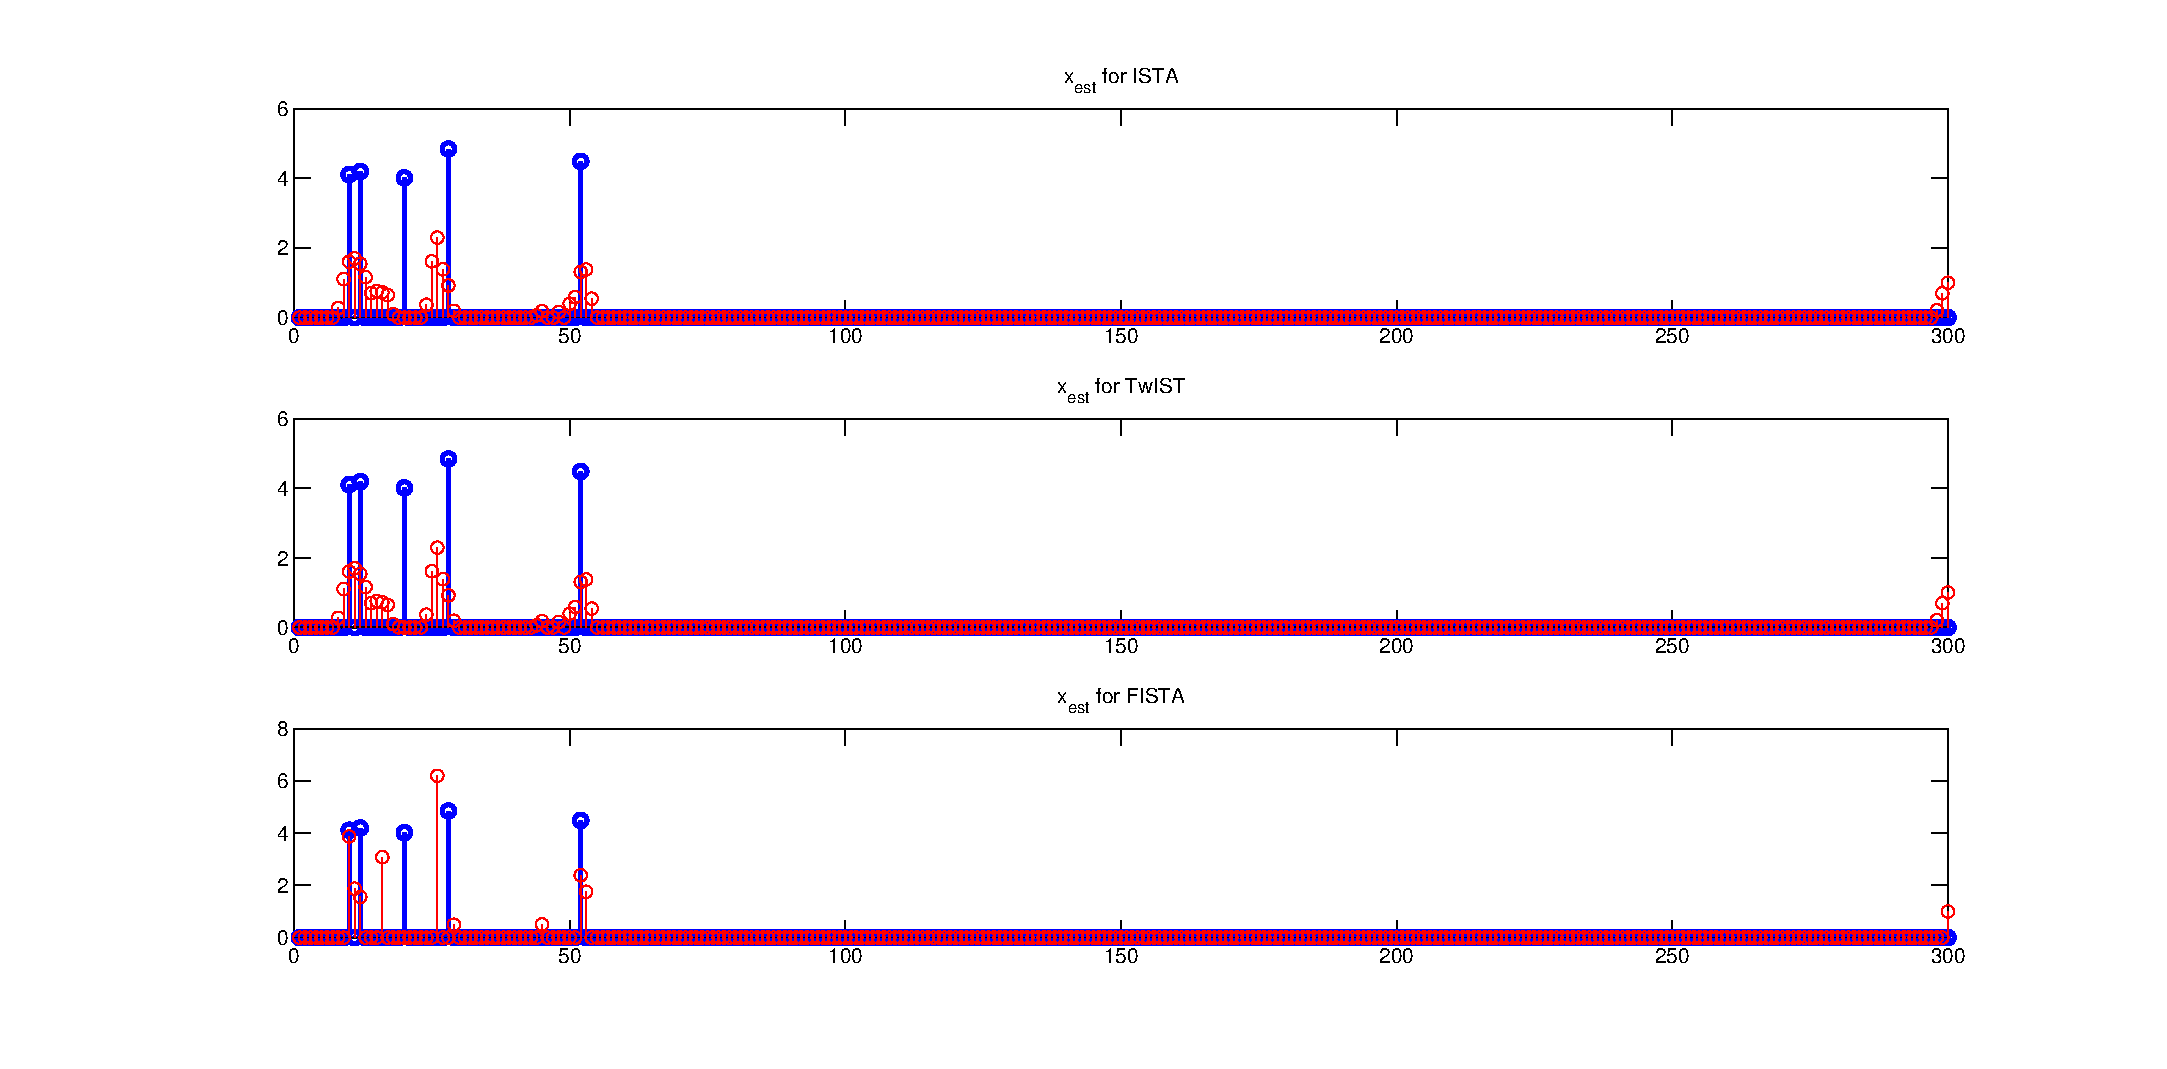
\includegraphics[trim = 10mm 10mm 10mm 0mm, clip,width=1.0\textwidth]{figs/Test_Image}
		\caption{CaptionName: Test Image from figs folder}
		\label{fig:Test}
	}
\end{figure}

% ***********************************************
\section{Conclusions}
\label{sec:Conclusions}

% ***********************************************
\nocite{*}  %Uncomment this line to print all citations 
\bibliographystyle{IEEEbib}
\bibliography{references} 

\end{document}